\documentclass[../notes.tex]{subfiles}

\pagestyle{main}
\renewcommand{\chaptermark}[1]{\markboth{\chaptername\ \thechapter\ (#1)}{}}
\setcounter{chapter}{9}

\begin{document}




\chapter{Isotope Effects}
\section{Thermodynamic Isotope Effects}
\begin{itemize}
    \item \marginnote{11/5:}Today.
    \begin{itemize}
        \item Finishing up transition state theory.
        \item Then how isotope effects can tell us stuff about reactions.
    \end{itemize}
    \item Lecture 16 recap.
    \begin{itemize}
        \item We defined an approach to kinetics.
        \item Basically, the \ce{A <=> B} equilibrium is decided by $\Delta G$ via
        \begin{equation*}
            \Keq = \e[-\Delta G/RT]
        \end{equation*}
        \item Then we can determine the rate at which this equilibrium is established viathe Eyring equation,
        \begin{equation*}
            k = \left( \kappa\frac{\kB T}{h} \right)\e[-\Delta G^\ddagger/RT]
        \end{equation*}
        \item Qualitative intuition for the relationship between the forms of the Eyring and equilibrium equations: TST is effectively analyzing a quasi-equilibrium between the SMs and the activated complex.
    \end{itemize}
    \item Lecture 16 continued.
    \item Let's think about the Eyring equation in terms of the entropies and enthalpies that make up $\Delta G^\ddagger$.
    \begin{align*}
        k &= \kappa\left( \frac{\kB T}{h} \right)\e[-\Delta H^\ddagger/RT]\cdot\e[\Delta S^\ddagger/R]\\
        \ln k &= \ln(\kappa\frac{\kB T}{h})-\frac{\Delta H^\ddagger}{R}\left( \frac{1}{T} \right)+\frac{\Delta S^\ddagger}{R}\\
        \ln(\frac{kh}{\kappa\kB T}) &= -\frac{\Delta H^\ddagger}{R}\left( \frac{1}{T} \right)+\frac{\Delta S^\ddagger}{R}
    \end{align*}
    \begin{itemize}
        \item These manipulations allow us to take the Eyring equation in slope-intercept form, so that we can linearize experimental data and extract from it experimental values for $\Delta H^\ddagger$ and $\Delta S^\ddagger$!
        \begin{itemize}
            \item This process is called forming an \textbf{Eyring plot}.
            \item If we can acquire data over a minimum temperature range of \SI{30}{\kelvin}, we can extrapolate reasonably accurate data.
        \end{itemize}
        \item Dick Zare at Stanford has some methods of observing activated complexes, but the main way of learning about them is indirectly through methods such as Eyring plots.
    \end{itemize}
    \item So using Eyring plots, we can get $\Delta H^\ddagger$ and $\Delta S^\ddagger$\dots but what do the values of these so-called activation parameters tell us?
    \item Qualitative interpretation of activation parameters.
    \begin{itemize}
        \item Typical Eyring plots have a negative slope.
        \begin{itemize}
            \item This means that we typically have $\Delta H^\ddagger>0$.
            \item This should make sense! Activated complexes have stretched out, weaker, higher energy bonds.
            \begin{itemize}
                \item The overwhelming majority of Eyring plots have said negative slopes due to said partial bonding.
            \end{itemize}
            \item Caveat: $\Delta H^\ddagger<0$ is physically possible, though uncommon.
            \begin{itemize}
                \item It corresponds to scenarios in which the activated complex is more enthalpically stable than the starting materials.
                \item There will be a question about a system with a negative enthalpy of activation on PSet 3!!
            \end{itemize}
        \end{itemize}
        \item Typical Eyring plots imply $\Delta S^\ddagger<0$.
        \begin{itemize}
            \item $\Delta S^\ddagger<0$ corresponds to an associative process.
            \item This is because degrees of freedom are being diminished in the activated complex, e.g., restricting rotation due to partial bonding.
            \item Example: The activated complex in a Diels-Alder reaction has an entropy of activation ($\Delta S^\ddagger$) of $-\eu{45}$.
            \begin{itemize}
                \item This is even higher than the \eu{30} we said we typically get in the van't Hoff analysis because we're restricting even more DOFs here, such as the rotation of dienophile.
            \end{itemize}
        \end{itemize}
        \item $\Delta S^\ddagger>0$ implies a dissociative process.
        \begin{itemize}
            \item Example: \ce{{}^{\emph{t}}BuO-O{}^{\emph{t}}Bu -> 2 {}^{\emph{t}}BuO*} has $\Delta S^\ddagger=\eu{11}$.
        \end{itemize}
        \item $\Delta S^\ddagger\approx 0$ implies an intramolecular process.
        \begin{itemize}
            \item Example: $4\pi$ retrocyclization of cyclobutene has $\Delta S^\ddagger=-\eu{1}\approx\eu{0}$.
            \item The error bars on these values are probably $\approx\eu{5}$, so don't read anything into the above value besides that it's "close to zero."
        \end{itemize}
    \end{itemize}
    \item Sometimes, big $\Delta G$ values (positive or negative) can affect reaction kinetics. Let's look at how.
    \item The interplay of thermodynamics and kinetics: A justification for the Hammond postulate.
    \item Let's first build a mathematical model for our justification.
    \begin{figure}[h!]
        \centering
        \begin{tikzpicture}[
            every node/.style=black
        ]
            \small
            \draw (-3,0) -- node[below=4.7mm]{Reaction Coordinate} (3,0);
    
            \footnotesize
            \node [below] {\ce{A***B***C}};
            \draw [grx,thick] (-2,3.5)
                to[out=-85,in=180,in looseness=0.5] (-1,0.5) node[below=5mm,xshift=-1cm]{\ce{A-B + C}}
                to[out=0,in=180,out looseness=0.5,in looseness=1.2] (2.8,3)
            ;
            \draw [grx,thick,xscale=-1] (-2,3.5)
                to[out=-85,in=180,in looseness=0.5] (-1,0.5) node[below=5mm,xshift=1cm]{\ce{A + B-C}}
                to[out=0,in=180,out looseness=0.5,in looseness=1.2] (2.8,3)
            ;
    
            \draw [grx,dashed] (-2.5,3.5) parabola bend (-1,0.5) (0.5,3.5);
            \draw [grx,dashed,xscale=-1] (-2.5,3.5) parabola bend (-1,0.5) (0.5,3.5);
        \end{tikzpicture}
        \caption{Bell-Evans-Polanyi principle: A model to visualize the principle.}
        \label{fig:BEPmodel}
    \end{figure}
    \pagebreak
    \begin{itemize}
        \item Consider a model reaction \ce{A-B + C <=> A + B-C}.
        \item \ce{A-B} has an anharmonic bond energy well, and we can think of the \ce{B-C} bond energy well as being mirror-reflected.
        \begin{itemize}
            \item These wells will have a depth on the order of a bond enthalpy, i.e., $\approx\kcal{70}$.
        \end{itemize}
        \item The two curves meet when \ce{A-B} is stretching and \ce{B-C} is stretching, i.e., in \ce{A***B***C}.
        \begin{itemize}
            \item This looks a lot like an activated complex!
        \end{itemize}
        \item The intersection point of these two curves is pretty far down.
        \begin{itemize}
            \item Recall from Table \ref{tab:energyRate} that for an activation energy to be viable, it has to be $<\kcal{25}$.
            \item Thus, since the well depth is $\approx\kcal{70}$ and the intersection point is pretty far down, we should be good to go.
        \end{itemize}
        \item But how do we calculate this intersection point?
        \begin{itemize}
            \item Although the wells aren't harmonic, we may approximate them reasonably well as parabolas.
            \item Then solving for the parabolic curve crossing intersection point is mathematically simple!
        \end{itemize}
    \end{itemize}
    \item Let's do parabolic curve crossing.
    \begin{figure}[h!]
        \centering
        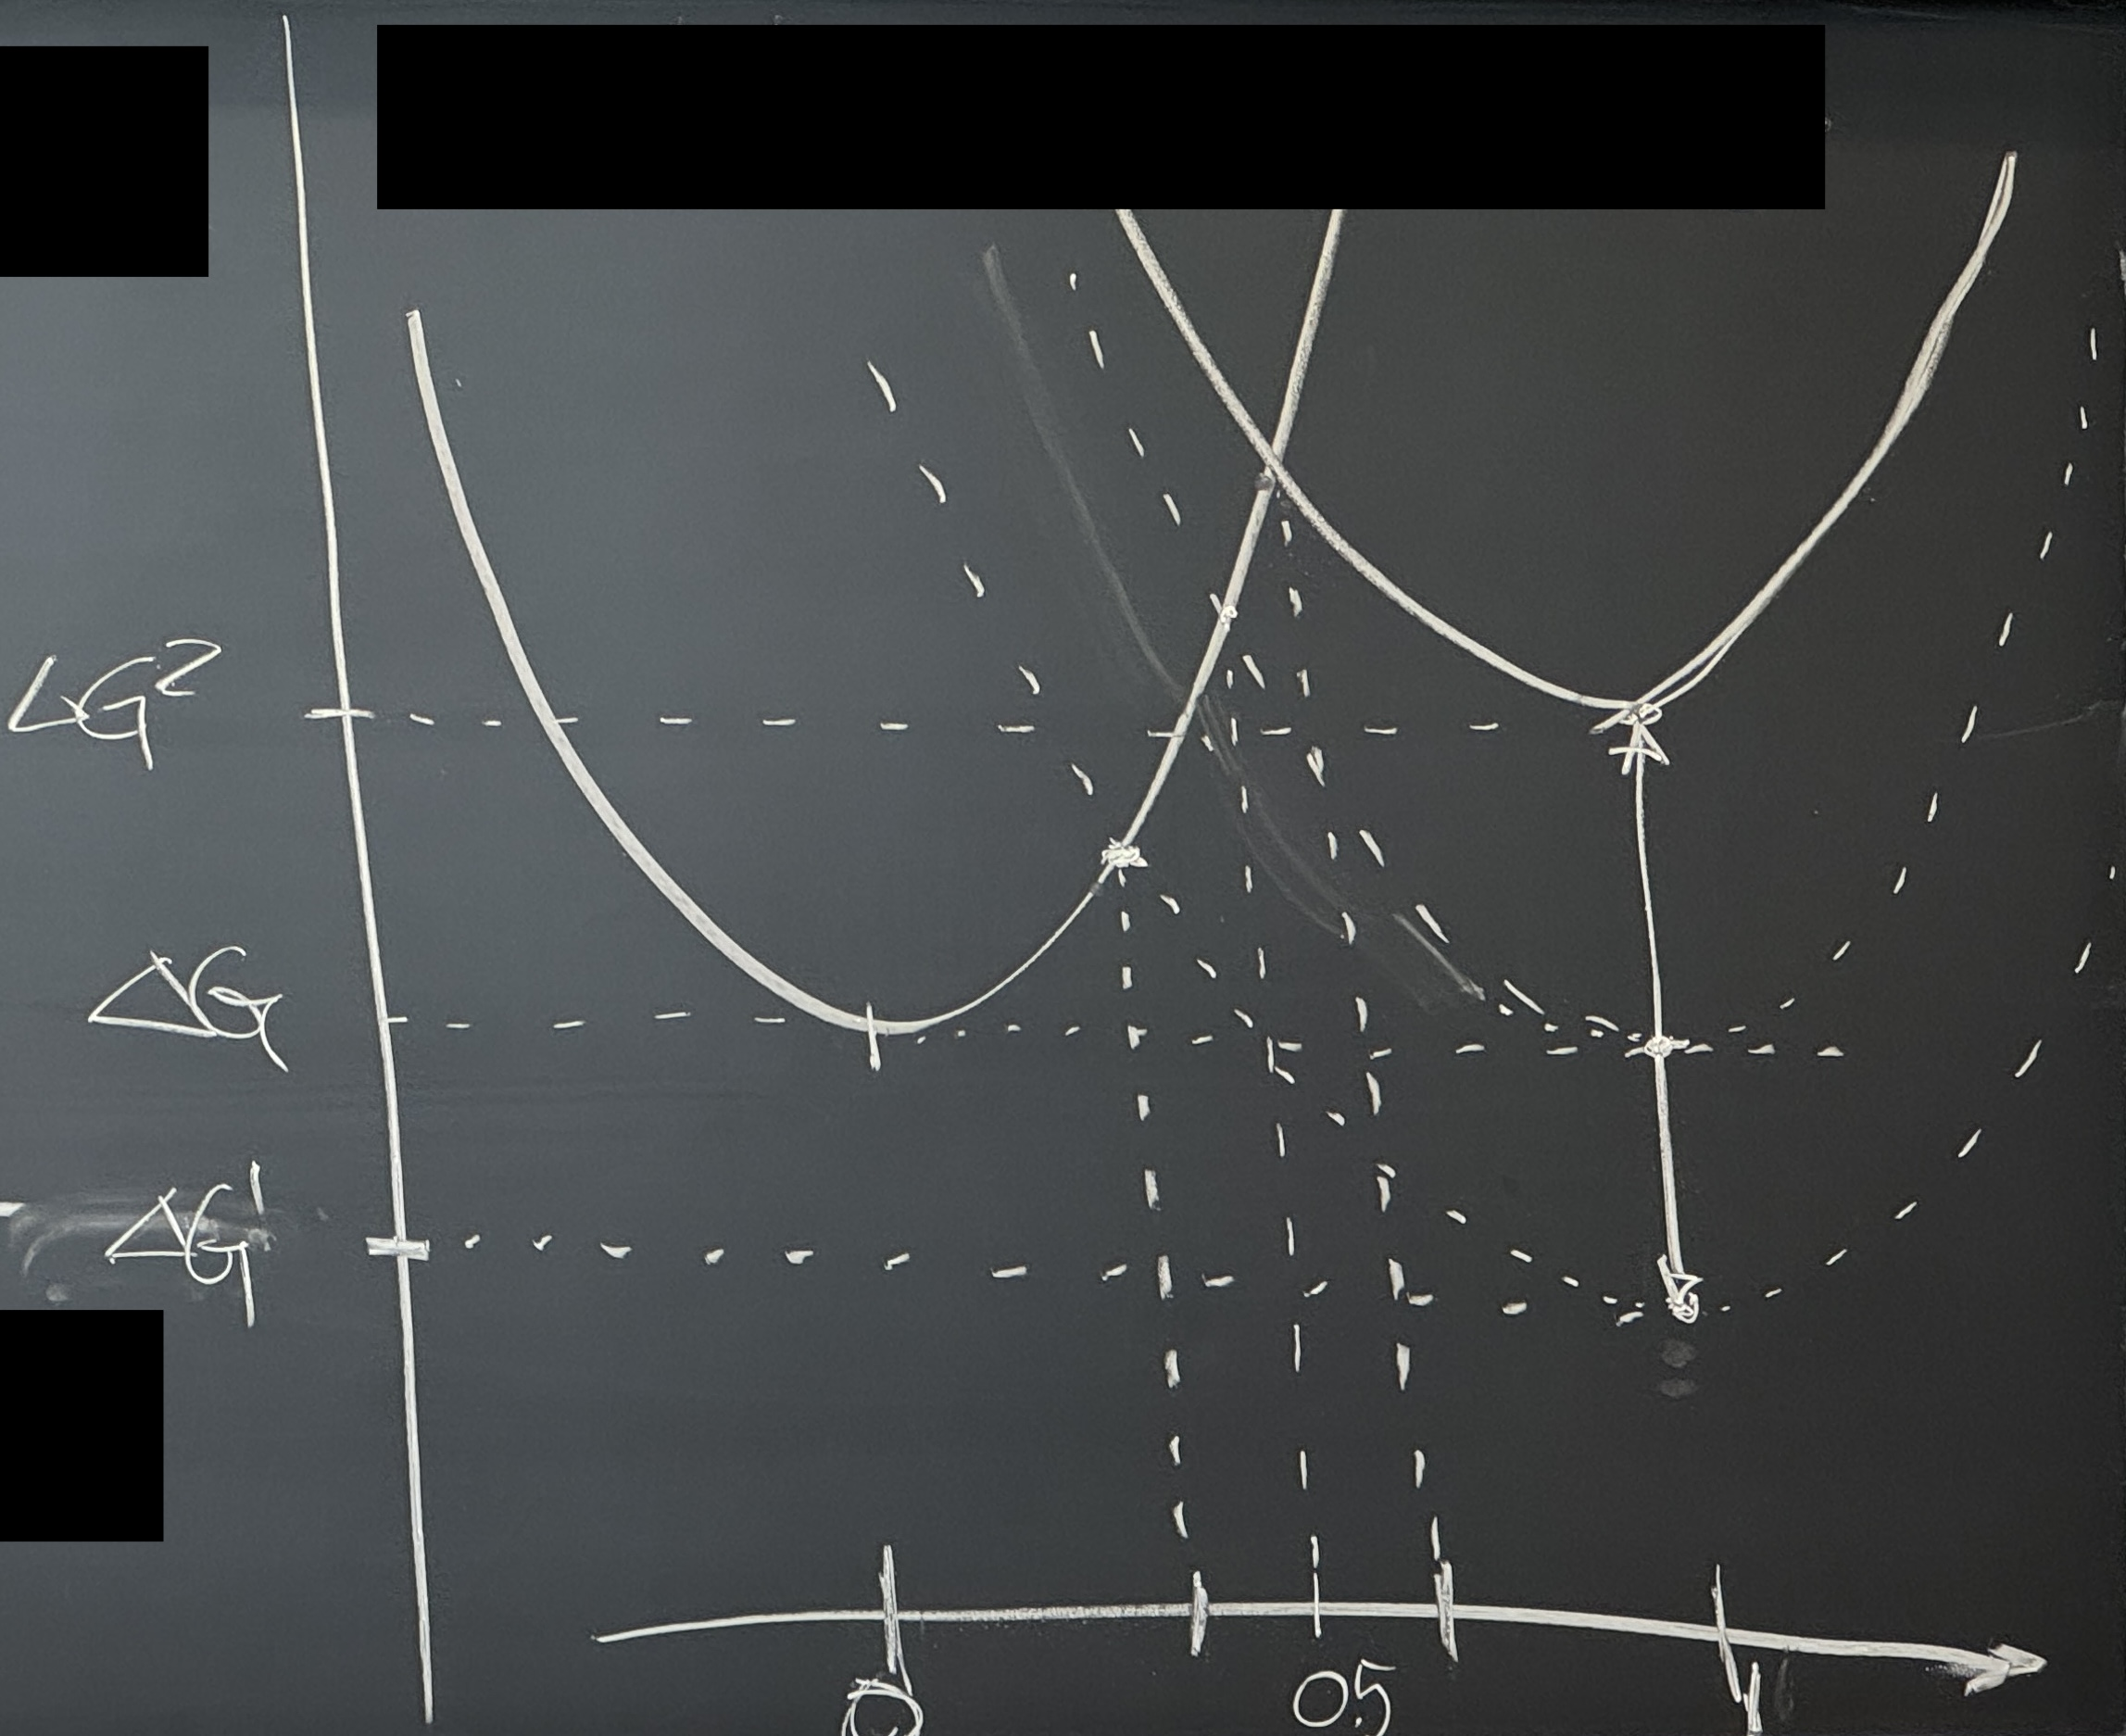
\includegraphics[width=0.4\linewidth]{BEPparabola.JPG}
        \caption{Bell-Evans-Polanyi principle: Parabolic curve crossing.}
        \label{fig:BEPparabola}
    \end{figure}
    \begin{itemize}
        \item Both parabolas should have the same curvature.
        \item Suppose first that the second vertex is lower in energy by $\Delta G^1$.
        \begin{itemize}
            \item This implies that the TST happens at less than 0.5 along the reacton coordinate.
            \item Implication: Exergonic reactions have TSTs lower in energy than the degenerate reaction, and with a TST more like the SMs ("earlier").
        \end{itemize}
        \item If $\Delta G^2>0$, endergonic reactions have a TST more like the products ("later") and higher energy.
        \item This is all collectively known in the literature as the \textbf{Bell-Evans-Polanyi principle}, or alternatively as the \textbf{Hammond postulate}.
    \end{itemize}
    \item Example: Radical halogenation of alkanes.\footnote{See Figure \ref{fig:Hammond} for where Masha covered this.}
    \begin{table}[H]
        \centering
        \small
        \renewcommand{\arraystretch}{1.2}
        \begin{tabular}{c|ccc}
             & \textbf{$\bm{1^\circ}$ \ce{C-H}} & \textbf{$\bm{2^\circ}$ \ce{C-H}} & \textbf{$\bm{3^\circ}$ \ce{C-H}}\\
            \hline
            \ce{F*}  & $1$ & $1.2$ & $1.4$\\
            \ce{Cl*} & $1$ & $3.9$ & $5$\\
            \ce{Br*} & $1$ & $82$  & $1600$\\
        \end{tabular}
        \caption{Relative reactivity rates in radical halogenation.}
        \label{tab:reactRadHalo}
    \end{table}
    \begin{itemize}
        \item Consider the reaction of \ce{F*}, \ce{Cl*}, and \ce{Br*} with primary, secondary, and tertiary \ce{C-H} bonds.
        \item Specifically, consider the relative rate $\krel$ of these reactions.
        \item Selectivity indicates that we should radically halogenate the tertiary \ce{C-H} first.
        \item Additionally, we observe drastically improved selectivity as we get to heavier halogens. Here's a quantitative explanation for this phenomenon.
        \begin{itemize}
            \item The reactants are at about \kcal{100} because that's the approximate \ce{R-H} bond enthalpy; see Masha's list!!
            \item Then \ce{Cl-H} is $\approx\kcal{103}$.
            \item For comparison, the \ce{H-Br} bond dissociation energy is $\approx\kcal{87}$.
        \end{itemize}
        \item Alex now esentially redraws Figure \ref{fig:Hammond}.
    \end{itemize}
    \item This concludes Lecture 16.
    \item We now begin Lecture 17: Isotope effects.
    \item Recall from your previous coursework in quantum mechanics that atomic-scale oscillators have quantized --- not classically continuous --- energies.
    \begin{figure}[h!]
        \centering
        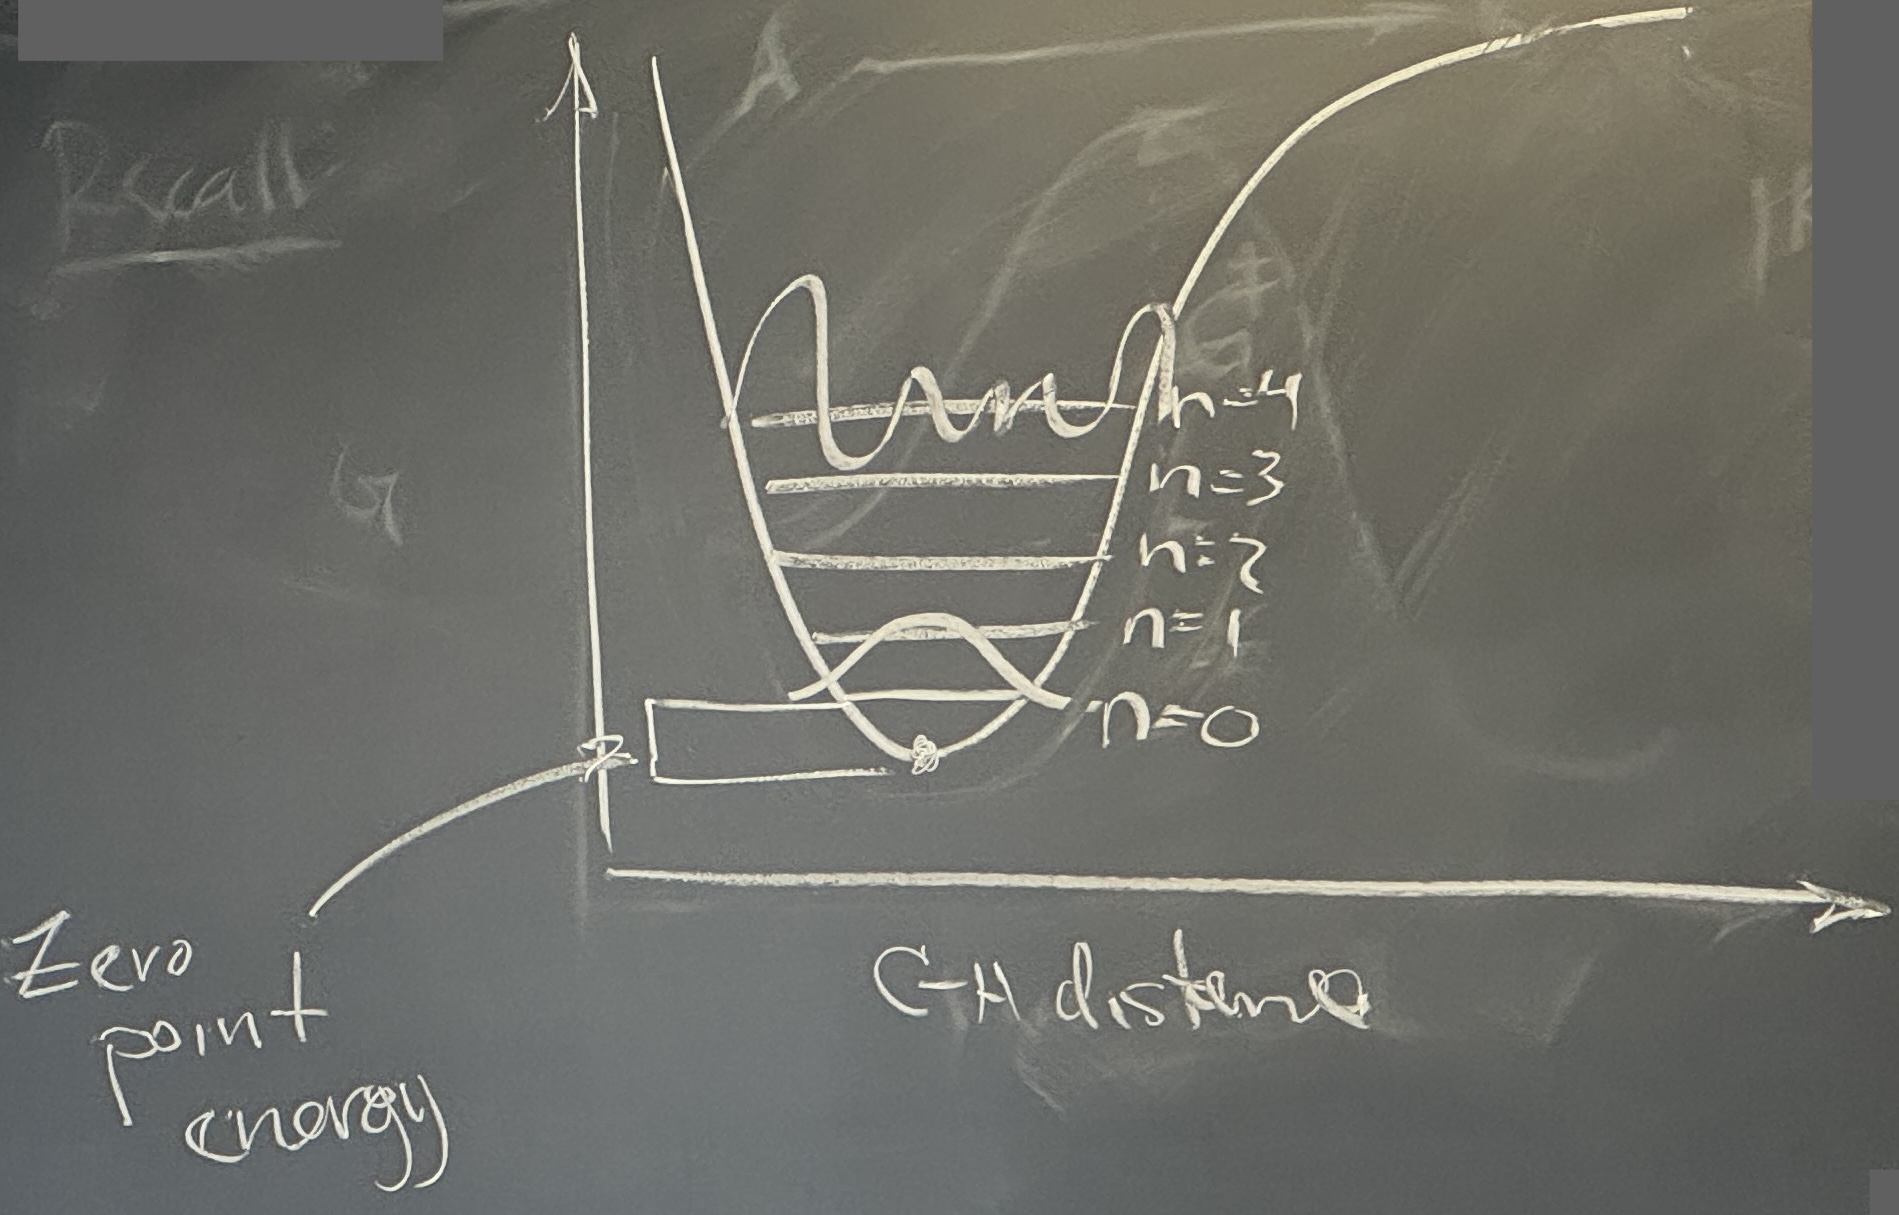
\includegraphics[width=0.5\linewidth]{quantumOsc.JPG}
        \caption{Quantum oscillator potential.}
        \label{fig:quantumOsc}
    \end{figure}
    \begin{itemize}
        \item So while we do have a minimum on the potential energy surface, the molecule does not hang out there because this would require that the quantum particle is static (so we'd know its position and momentum, violating Heisenberg uncertainty).
        \item So at the energy minimum, there is residual energy latent in the system called \textbf{zero-point energy}.
        \item So even in the lowest wave function, there's gonna be some spread of the nuclear position beyond the potential well.
    \end{itemize}
    \item \textbf{Zero-point energy}. \emph{Also known as} \textbf{ZPE}.
    \item Quantized vibrational energies.
    \begin{table}[h!]
        \centering
        \small
        \renewcommand{\arraystretch}{1.2}
        \begin{tabular}{cc}
            \textbf{Bond} & $\bm{\mu}$\\
            \hline
            \ce{C-H}           & $0.92$\\
            \ce{C-D}           & $1.72$\\
            \ce{{}^12C-{}^12C} & $6.00$\\
            \ce{{}^12C-{}^13C} & $6.24$\\
        \end{tabular}
        \caption{The reduced mass of common chemical bonds.}
        \label{tab:redMassBond}
    \end{table}
    \begin{itemize}
        \item We have that
        \begin{equation*}
            E_n = h\nu\left( n+\frac{1}{2} \right)
        \end{equation*}
        \item Recall that an (asymmetric) molecule has $3N-6$ vibrational modes.
        \item This frequency of oscillation (per Hooke's law) is related to the force constant and \textbf{reduced mass}.
        \begin{equation*}
            \nu = \frac{1}{2\pi}\sqrt{\frac{k}{\mu}}
        \end{equation*}
        \item Atoms are defined by the number of protons, but we can change the number of neutrons as much as we want! This will change the reduced mass.
        \item The magnitude of isotope effects is the greatest when the reduced mass changes the most.
    \end{itemize}
    \item \textbf{Reduced mass}: The quantity given as follows, where $m_1,m_2$ are the masses of two particles in a system. \emph{Denoted by} $\bm{\mu}$. \emph{Given by}
    \begin{equation*}
        \mu = \frac{m_1m_2}{m_1+m_2}
    \end{equation*}
    \item Looking at the deuterium isotopologue vs. carbon.
    \begin{figure}[h!]
        \centering
        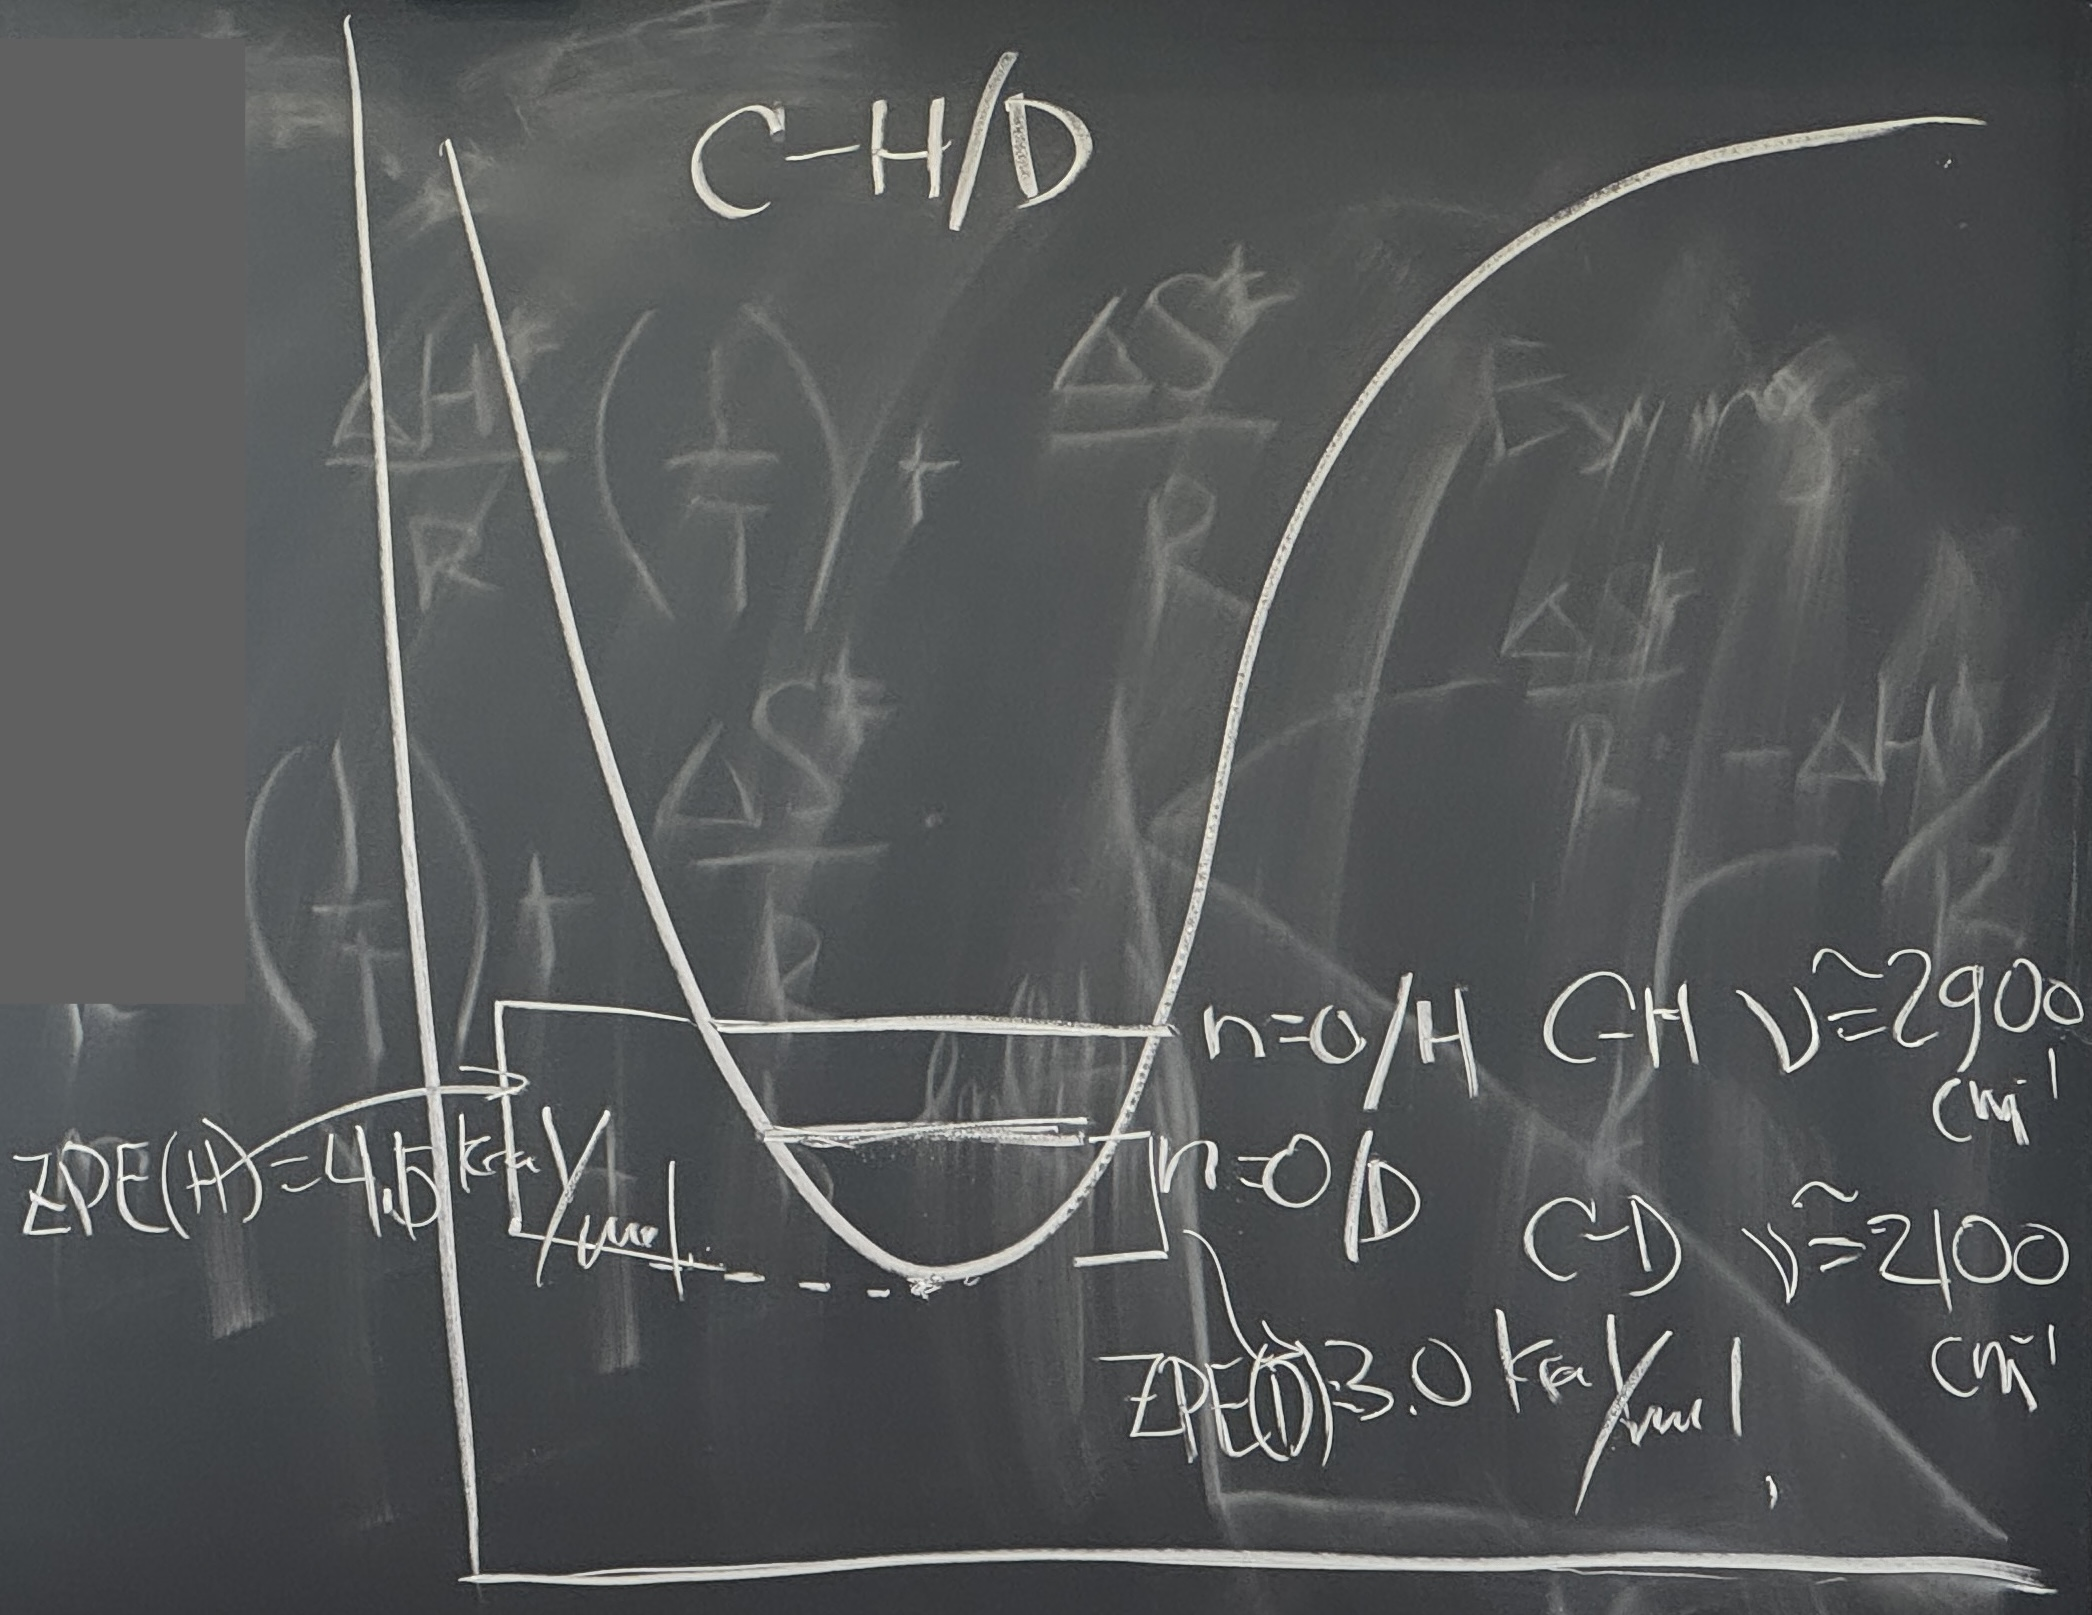
\includegraphics[width=0.45\linewidth]{quantumIso.JPG}
        \caption{Isotopic differences alter the thermodynamic stability of a chemical bond.}
        \label{fig:quantumIso}
    \end{figure}
    \begin{itemize}
        \item The zero-point energy for the \ce{C-D} oscillator is less than for the \ce{C-H} operator.
        \item Thus, \ce{C-H} has $\nu\approx\SI{2900}{\per\centi\meter}$ and \ce{C-D} has $\nu\approx\SI{2100}{\per\centi\meter}$.
        \item This means that it will cost more energy to dissociate a \ce{C-D} bond vs. a \ce{C-H} bond.
        \item The potential is defined only by positive and negative charges, so \emph{it's} the same; it's only the isotopes within it that change.
        \item The zero-point energy of a \ce{C-H} bond is \kcal{4.5}, and the zero-point energy of a \ce{C-D} bond is \kcal{3.0}.
        \item These \kcal{1.5} impact the kinetics reactivity by about sevenfold!
    \end{itemize}
    \pagebreak
    \item Equilibrium isotope effects.
    \begin{figure}[h!]
        \centering
        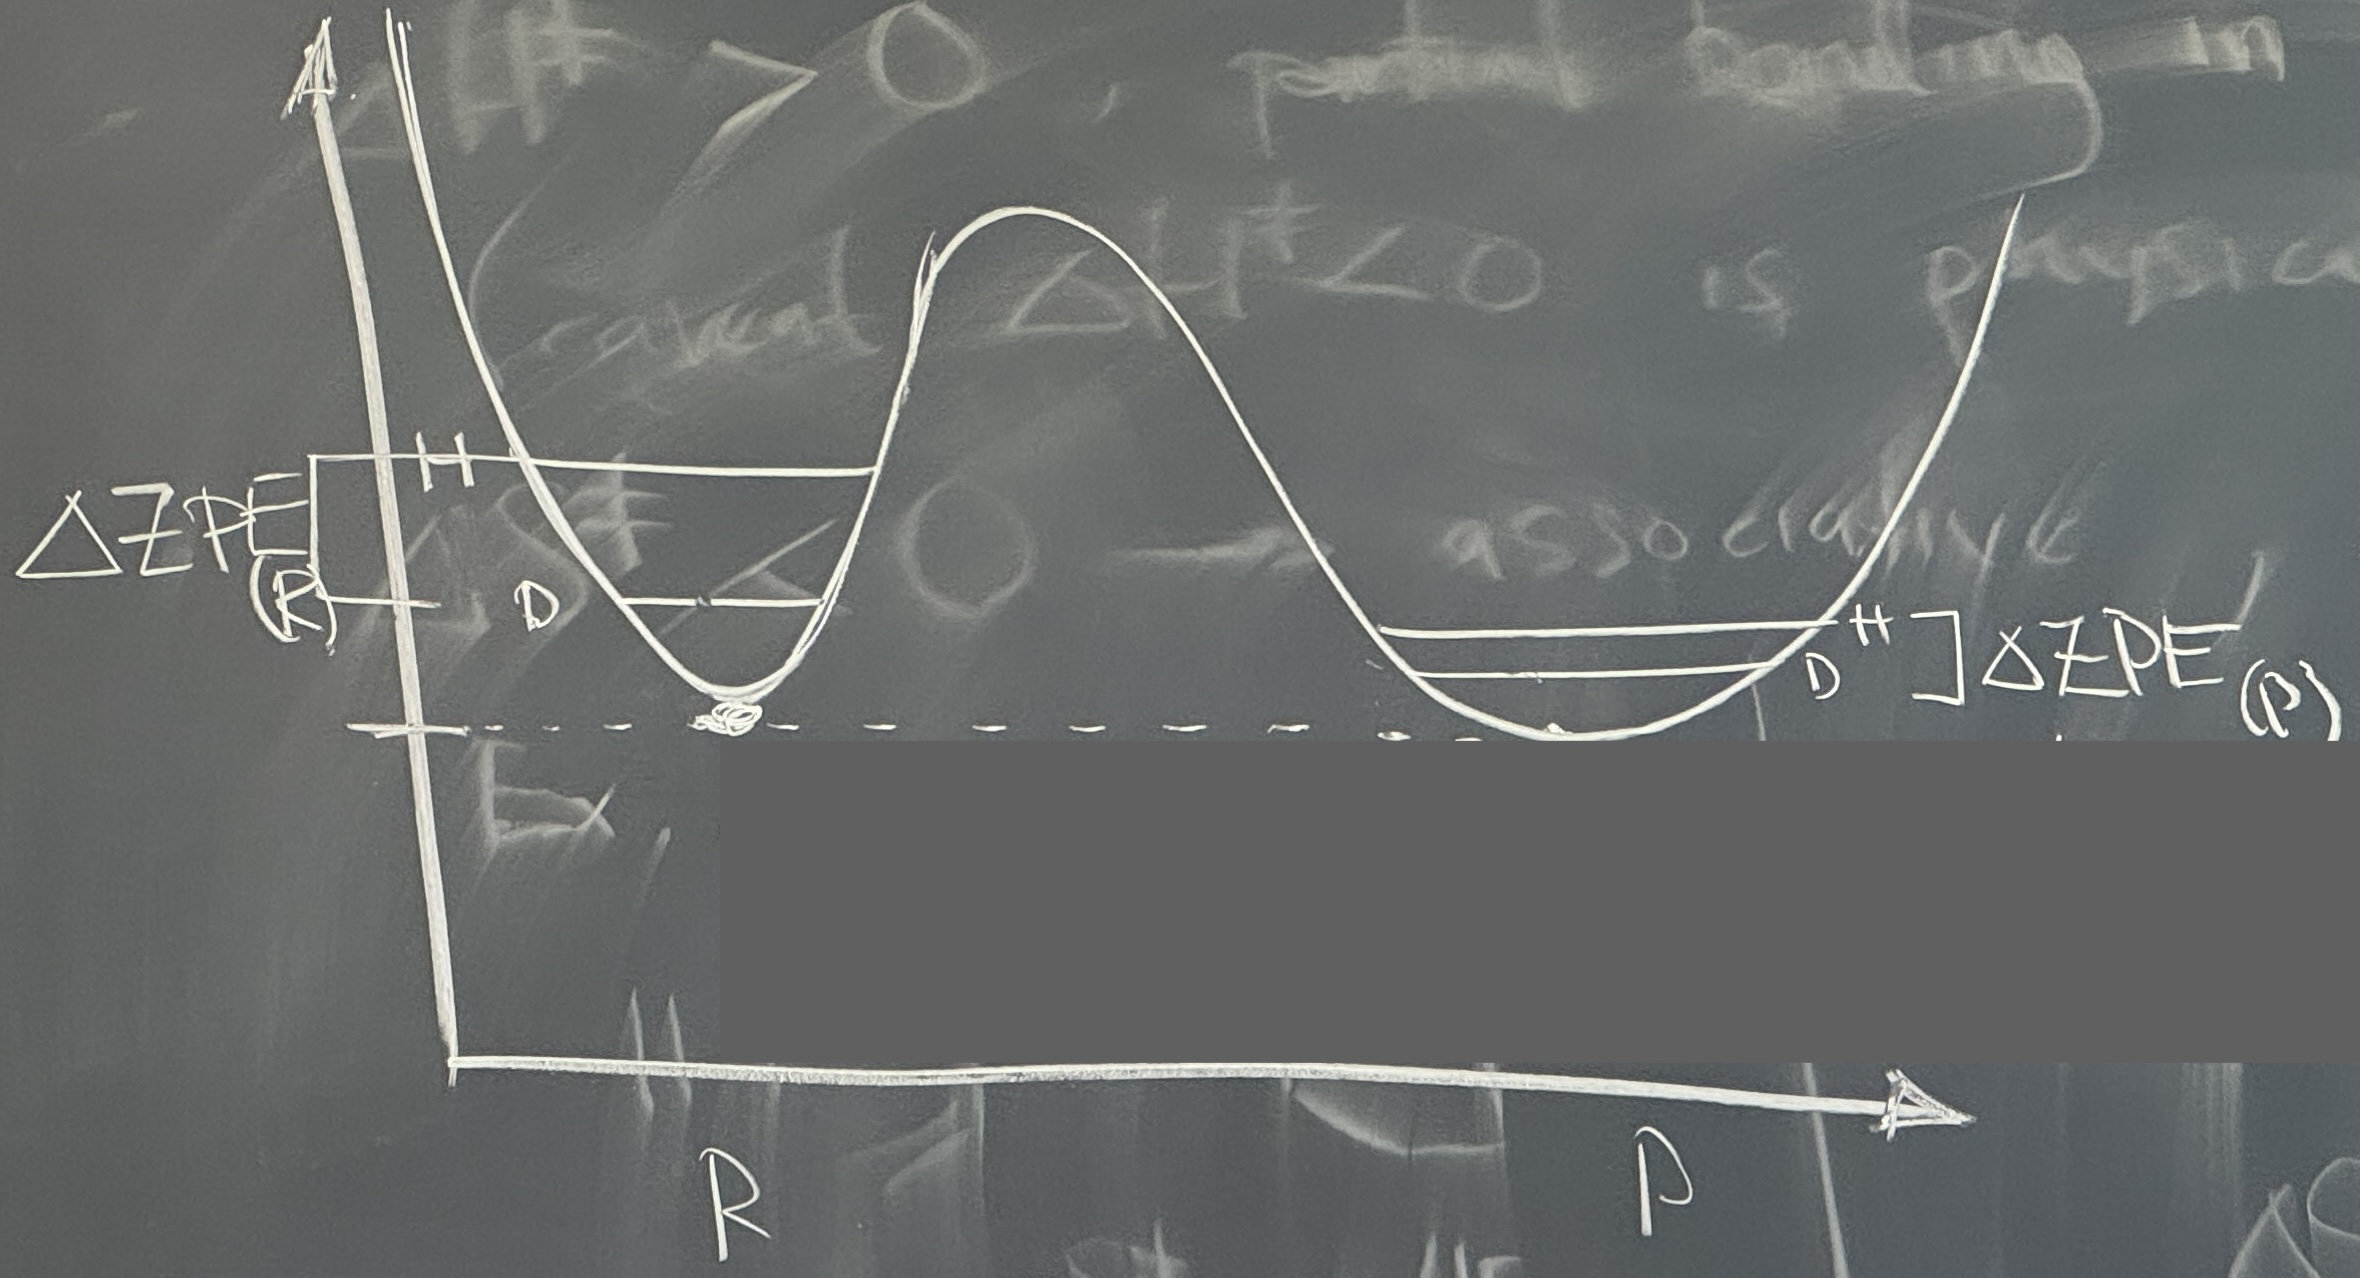
\includegraphics[width=0.55\linewidth]{isotopeEq.JPG}
        \caption{Equilibrium isotope effects.}
        \label{fig:isotopeEq}
    \end{figure}
    \begin{itemize}
        \item Consider an energetically degenerate reaction.
        \item Suppose that the difference in ZPEs is smaller in the products' slack potential.
        \begin{itemize}
            \item Symbolically, $\Delta\ZPE_\text{(R)}>\Delta\ZPE_\text{(P)}$.
        \end{itemize}
        \item So the effective $\Delta G$ for \ce{H} is greater than the one for \ce{D}: $-\Delta G_{\ce{H}}>-\Delta G_{\ce{D}}$.
        \begin{itemize}
            \item Thus, $k_{\ce{H}}/k_{\ce{D}}>1$.
        \end{itemize}
    \end{itemize}
    \item Example: Equilibrium isotope effects during reductive elimination/oxidative addition at transition metals.
    \begin{figure}[h!]
        \centering
        \footnotesize
        \schemestart
            \chemfig{L_nM@{}{}^{n+2}(-[1,,2]CH_3)(-[7,,2]H/D)}
            \arrow{<=>}
            \chemfig{L_nM}
            \arrow{0}[,0.1]\+{,,-1.2em}
            \chemfig{CH_3-[6]H@{}/D}
        \schemestop
        \caption{Reductive elimination of methane.}
        \label{fig:redElimCH4}
    \end{figure}
    \begin{itemize}
        \item Consider a generic metal-ligand complex (\ce{L_nM}) undergoing the reaction in Figure \ref{fig:redElimCH4}.
        \item The typical BDE for a \ce{M-H} bond is \kcalr{40}{80}.
        \begin{itemize}
            \item The BDE for a methane \ce{H_3C-H} bond is \kcal{104}.
        \end{itemize}
        \item Since the metal potential is shallower, it is slacker and hence has a lower associated force constant.
        \begin{itemize}
            \item Symbolically, $k_{\ce{M-H}}<k_{\ce{C-H}}$.
        \end{itemize}
        \item Since the ZPE difference is smaller in the more slack potential (per Figure \ref{fig:isotopeEq}), it follows that
        \begin{equation*}
            \Delta\ZPE_{\ce{M-H/D}} < \Delta\ZPE_{\ce{C-H/D}}
        \end{equation*}
        \item Takehome: Deuterated species prefer to be in the well with the stronger force constant.
    \end{itemize}
    \item Accounting for the anharmonicity\footnote{How is this related to anharmonicity??} in the potential wells.
    \begin{figure}[H]
        \centering
        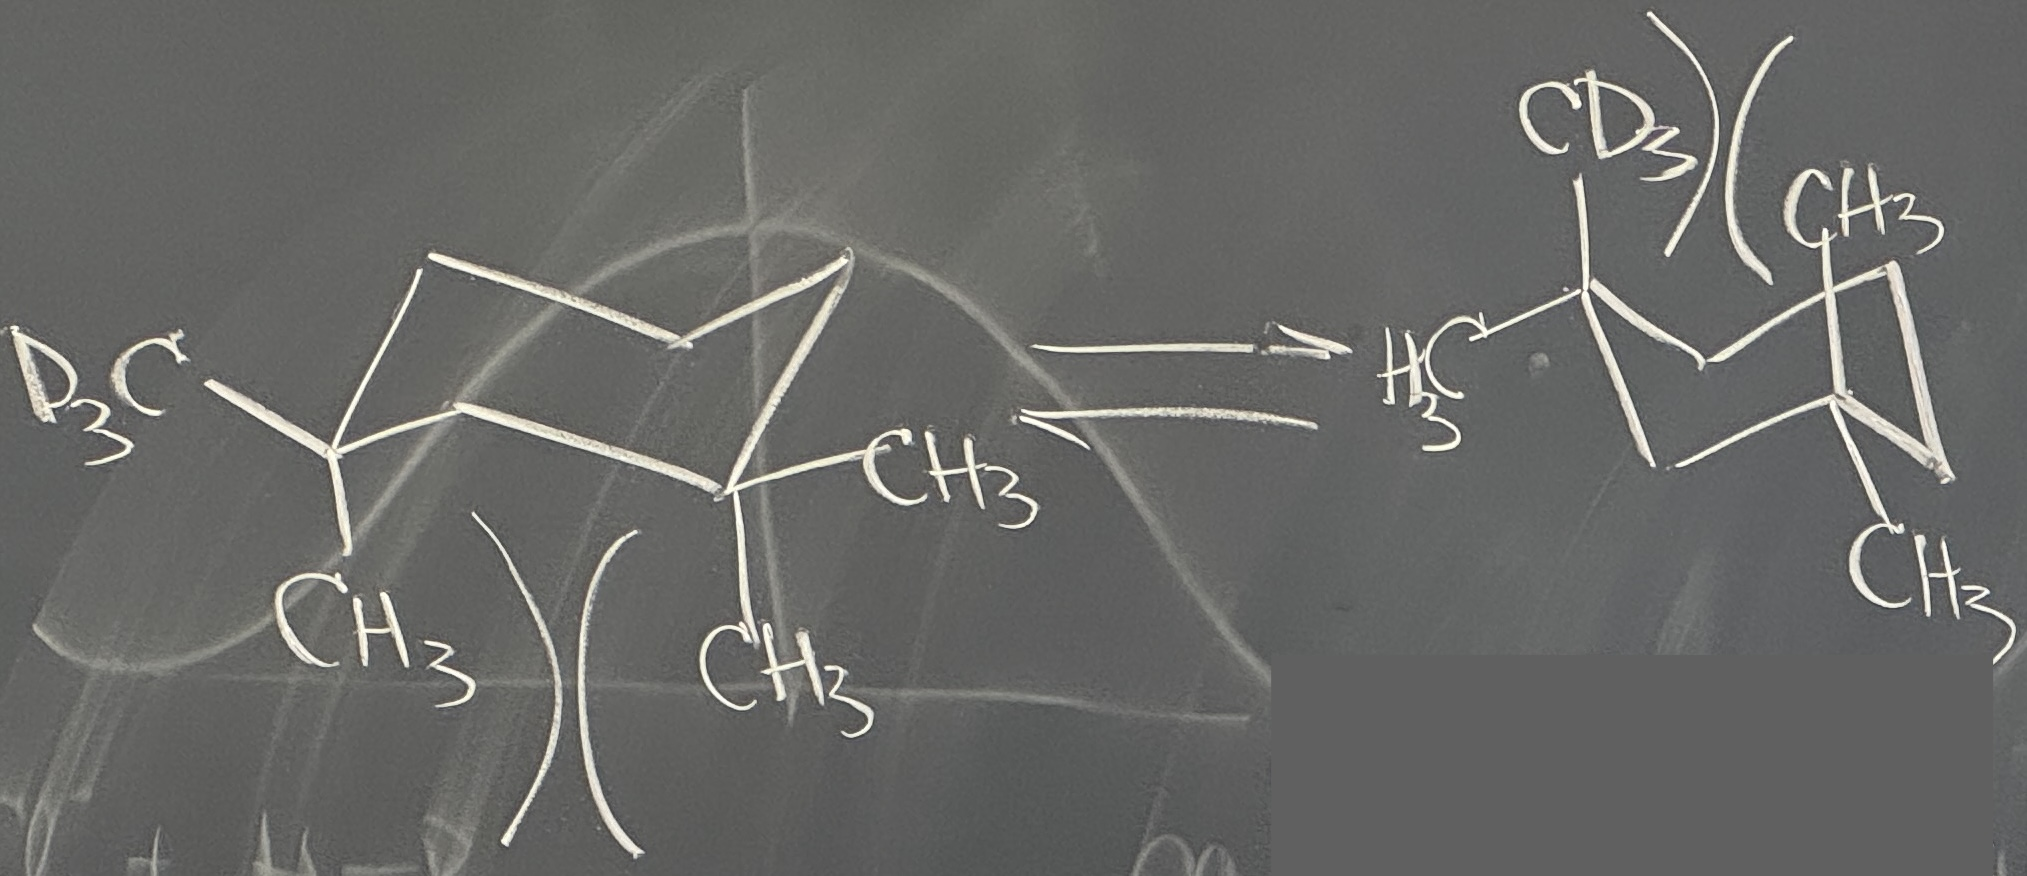
\includegraphics[width=0.35\linewidth]{isotopeSteric.JPG}
        \caption{Steric isotope effects.}
        \label{fig:isotopeSteric}
    \end{figure}
    \begin{itemize}
        \item Consider the ring flip of 1,1,3,3-tetramethylcyclohexane, with one of the methyl groups actually a \ce{CD3} group.
        \item Experimentally, we observe that
        \begin{equation*}
            K = \frac{\cnc{CD3 ax}}{\cnc{CD3 eq}} = 1.042
        \end{equation*}
        at $-\SI{100}{\celsius}$.
        \item It is preferable to have the \ce{CD3} group axial because it is smaller: The lower vibrational amplitude $\nu$ for \ce{C-D} bonds relative to \ce{C-H} bonds literally shrinks the sterics of the group \parencite[430,434]{bib:Anslyn}.
    \end{itemize}
    \item How can we link equilibrium isotope effects to kinetics?
    \begin{itemize}
        \item Like at the beginning of class, we use transition state theory!
        \item Indeed, let's apply our understanding of equilibrium isotope effects to the quasi-equilibrium between the starting materials and transition state. This can give us valuable insight into the relative rates of reaction for heavier vs. lighter isotopologues.
    \end{itemize}
    \item Kinetic isotope effects.
    \begin{figure}[h!]
        \centering
        \begin{tikzpicture}[
            every node/.style=black
        ]
            \small
            \draw [stealth-stealth] (0,4) -- (0,0) -- (7,0);
            \node [below] at (1.5,0) {\ce{C-H + *X}};
            \node [below] at (4,0) {$[\ce{C***H***X}]^\ddagger$};
            \node [below] at (6.5,0) {\ce{C* + H-X}};
    
            \footnotesize
            \draw [grx,thick,name path=PES] (0.3,3.8)
                to[out=-85,in=180,in looseness=0.7] (1.5,0.8)
                to[out=0,in=180,out looseness=0.7] (4,3.2)
                to[out=0,in=180,in looseness=0.6] (6.5,0.1)
                to[out=0,in=-150,out looseness=0.6] (6.8,0.2)
            ;
    
            \footnotesize
            \path [name path=CH] (0.5,1.3) -- ++(2,0);
            \draw [grx,name intersections={of=PES and CH}] (intersection-1) node[left]{\ce{C-H}} -- (intersection-2);
            \path [name path=CD] (0.5,1.0) -- ++(2,0);
            \draw [grx,name intersections={of=PES and CD}] (intersection-1) node[left]{\ce{C-D}} -- (intersection-2);
            \draw [|-|] (2.4,1) -- node[right]{$\Delta\ZPE_\text{(GS)}^{\textcolor{white}{(GS)}}$} ++(0,0.3);
    
            \filldraw [grx,thick,name path=PESo1] (4,3.2) to[out=180,in=-30] (2.5,3.57) -- (2.5,3.63) to[out=-30,in=180] cycle;
            \draw [grx,thick,dashed,name path=PESo2] (4,3.2) to[out=0,in=-150] (5.5,3.6);
            \path [name path=CH] (2.5,3.4) -- ++(3,0);
            \draw [grx,name intersections={of=PESo1 and CH},name intersections={of=PESo2 and CH}] (intersection-2) node[above left=-2pt,xshift=-5mm]{\ce{C-H}} -- (intersection-1);
            \path [name path=CD] (2.5,3.3) -- ++(3,0);
            \draw [grx,name intersections={of=PESo1 and CD},name intersections={of=PESo2 and CD}] (intersection-2) node[below left=-2pt]{\ce{C-D}} -- (intersection-1);
            \draw [|-|] (5.5,3.3) -- node[right]{$\Delta\ZPE_\text{(TS)}^{\textcolor{white}{(TS)}}$} ++(0,0.1);
        \end{tikzpicture}
        \caption{Kinetic isotope effects.}
        \label{fig:KIE}
    \end{figure}
    \begin{itemize}
        \item Consider the HAT reaction
        \begin{equation*}
            \ce{C-H + *X -> C* + H-X}
        \end{equation*}
        \begin{itemize}
            \item This is a nondegenerate reaction, energetically.
        \end{itemize}
        \item Recall that transition structures are maxima along one direction, but minima along every other direction in the hyperspace (see Figure \ref{fig:EDtBuClcon}).
        \begin{itemize}
            \item It follows that $\Delta\ZPE$ is relatively small in the TS, because TS potentials are pretty slack compared with bond potentials.
        \end{itemize}
        \item The important equation we can write from the above diagram is
        \begin{equation*}
            \Delta\Delta G^\ddagger = \Delta\Delta\ZPE
            = \Delta\ZPE_\text{(GS)}-\Delta\ZPE_\text{(TS)}
        \end{equation*}
        \begin{itemize}
            \item This means that it's easier to take \ce{C-H} to the transition state than \ce{C-D}.
            \item This is a \textbf{normal KIE}, where $k_{\ce{H}}/k_{\ce{D}}>1$.
            \item This is also primary ($1^\circ$) because the isotope-sensitive bond is the one being broken/made.
        \end{itemize}
    \end{itemize}
    \item \textbf{Inverse KIEs} involve cases in which $k_{\ce{D}}/k_{\ce{H}}<1$.
    \begin{itemize}
        \item This is also $1^\circ$.
    \end{itemize}
    \item We can also have \textbf{secondary} KIEs, where we label a position potentially far from the reactive site.
    \item Next time: Using KIEs to diagnose reaction mechanisms, single isotopologues under different reaction conditions give us different information, etc. Takeaways: KIEs are super useful.
\end{itemize}




\end{document}